\section{Programa de Pós-Graduação em Ciência da Computação}

O Programa de Pós-Graduação em Ciência da Computação (PGCOMP) da Universidade Federal da Bahia (UFBA), aprovado pela CAPES, oferece os cursos de Mestrado em Ciência da Computação e de Doutorado em Ciência da Computação, com o objetivo de dar suporte à formação de pesquisadores com competência para gerar novos conhecimentos, conduzir projetos de investigação científica e exercer atividades de docência no Ensino Superior (graduação e pós-graduação lato sensu e stricto sensu) nas áreas de Ciência da Computação e Tecnologia da Informação e Comunicação (TIC).

\subsection{Grupos de Pesquisa}

A maior parte da pesquisa realizada no DCC está ligada aos cursos de pós-graduação apoiados e ao 
    seu corpo docente, atuante em diversas áreas, linhas, grupos de pesquisa, que dentre outros são os seguintes:

\subsubsection{Laboratorio de Sistemas Distribuídos} 
\begin{wrapfigure}{R}{0.3\textwidth}
            \centering
            
\includegraphics[scale = 0.4]{logolasid.png}
        \end{wrapfigure}  
O Laboratório de Sistemas Distribuídos ( LaSiD) é um laboratório de pesquisa dentro do Departamento de Ciência da Computação na Universidade Federal da Bahia (UFBA) . Trata-se de membros do corpo docente do Departamento de Ciência da Computação , assistentes de pesquisa e estudantes de pesquisa ( Ph.D, MSc. E Licenciatura). A missão da LaSiD é desenvolver métodos, técnicas e ferramentas que ajudam na concepção de sistemas distribuídos corretas e confiáveis, a preparar a próxima geração de pesquisadores e desenvolvedores nestas áreas por investigar problemas desafiadores.
\newline
\newline
\newline
\newline\subsubsection{Laboratório de Engenharia de Software}
\begin{wrapfigure}{R}{0.3\textwidth}
            \centering
            
\includegraphics[scale = 0.4]{les.jpg}
        \end{wrapfigure}

O objetivo do Laboratório de Engenharia de Software da Universidade Federal da Bahia ( LES- UFBA) é estudar a disciplina de engenharia de software , bem como áreas que impactam a maneira como se desenvolve, mantém e gerencia software. LES tem vários grupos de pesquisa que investigam diferentes sub-áreas de engenharia de software.


\subsubsection{Web and Interactive Systems Research Group}
\begin{wrapfigure}{R}{0.3\textwidth}
            \centering
            
\includegraphics[scale = 0.2]{logoWISER.png}
        \end{wrapfigure}
O grupo realiza pesquisas nas áreas de Internet e Web voltadas para Web Semântica, Sistemas de Recomendação para Web, Serviços Web, Computação em Nuvem, Web e Internet das Coisas, Internet do Futuro, Recuperação da Informação na Web, Sistemas Interativos, Cidades Inteligentes e Tecnologias Assistivas. O grupo participou e participa de projetos em colaboração com outras instituições nacionais e internacionais.

\subsubsection{Inteligent Vision Research Lab}
\begin{wrapfigure}{R}{0.3\textwidth}
            \centering
            
\includegraphics[scale = 0.4]{logo_ivision.png}
        \end{wrapfigure}
As principais áreas de investigação Vision Lab estão em sistemas interactivos , detecção de objetos , imagem desempenho da classificação , compreensão cena em imagens , avaliação de classificadores de imagens , reconhecimento de ação , entre outros performance. Todas as pesquisas abrangem os campos de Cidades Inteligentes , Sistemas Inteligentes de Transporte e Sistemas biométricos.
	  
	  Um importante objetivo do laboratório é fornecer aplicações do mundo real; para isso, arquiteturas paralelas também estão sendo investigados , a fim de acelerar os sistemas propostos . Sob essa perspectiva , nós dirigimos a nossa pesquisa de requisitos acadêmicos para as necessidades da indústria , da visão a relação integrativa entre estes dois mundos.


\subsubsection{Software Desing and Evolution Group}
\begin{wrapfigure}{R}{0.3\textwidth}
            \centering
            
\includegraphics[scale = 0.4]{desig.jpg}
        \end{wrapfigure}
O design de software requer esforço e inteligência de pessoas para a criação de artefatos de software idealmente concebidos para realizar funções úteis para pessoas. E software útil está em constante evolução. Nesse contexto, o grupo de pesquisa aSide @UFBA tem como objetivo investigar aspectos da ``ciência do artificial'' e de seus processos de design e evolução de software, buscando caracterizar, desenvolver e avaliar modelos, princípios, práticas e ferramentas para que pessoas possam criar, desenhar, construir, validar, reutilizar, modificar, analisar, gerenciar e desfrutar de software de qualidade. 
	  
	  O aSide @ UFBA é um grupo de pesquisa certificado pela UFBA no Diretório de Grupos do CNPq e está associado ao Laboratório de Engenharia de Software (LES) da UFBA.


\subsubsection{Context and Ubiquitous Systems Group CEManTIKA}
\begin{wrapfigure}{R}{0.3\textwidth}
            \centering
            
\includegraphics[scale = 0.8]{cemantica.jpg}
        \end{wrapfigure}
O Grupo CEManTIKA visa estudar conceitos, técnicas, modelos e ferramentas que apoiem a construção de sistemas sensíveis ao contexto. São objetivos do grupo: 

\begin{itemize}
\item Desenvolver sistemas sensíveis ao contexto voltados para diferentes áreas; 
\item  Formalizar conceitos e metamodelos para modelagem de informações de contexto; 
\item  Investigar algoritmos e técnicas de apoio ao processamento do contexto usando raciocínio lógico; 
\item Desenvolver ferramentas de apoio ao projeto e implementação de sistemas sensíveis ao contexto. 
\end{itemize}

\subsubsection{Formalisms and Semantic Applications Research Group}
\begin{wrapfigure}{R}{0.3\textwidth}
            \centering
            
\includegraphics[scale = 0.4]{formas.jpg}
        \end{wrapfigure}
Objetivo principal é estudar , analisar e avaliar abordagens semânticas , cobrindo desde formalismos através de aplicações . As nossas principais áreas de investigação do grupo baseiam-se em cinco etapas principais em conseguir semântica: Métodos , ontologia, Extração de Informação , a interoperabilidade e validação formal . Lamentamos profundamente analisar cada uma dessas abordagens com foco na obtenção de altos níveis de compreensão semântica e pragmática.


\subsubsection{Grupo de Algoritmos e Computação Distribuida Gaudi}
\begin{wrapfigure}{R}{0.3\textwidth}
            \centering
            
\includegraphics[scale = 0.4]{gaudi.jpg}
        \end{wrapfigure}

O GAUDI visa o entendimento dos problemas fundamentais que surgem na confecção de sistemas e aplicações computacionais e a busca de soluções para os mesmos. A sua principal linha de pesquisa concentra-se no estudo de algoritmos distribuídos e na sua aplicação para o desenvolvimento de componentes de software que facilitem a construção de sistemas confiáveis. 

Linhas de Pesquisa: Algoritmos Distribuídos, Tolerância a Falhas, Componentes Distribuídos, Grades Computacionais, Redes Móveis Ad-Hoc (Manets), Teoria dos Grafos.

\subsubsection{Formal Meethods in Software Engineering Group}
\begin{wrapfigure}{R}{0.3\textwidth}
            \centering
            
\includegraphics[scale = 0.4]{MEFES.jpg}
        \end{wrapfigure}
Visa a proposição de processos de desenvolvimento de softwares que sejam sistemáticos, baseados em métodos e ferramentas, e aplicáveis a sistemas reais. Tendo sempre em mente a produção de software de qualidade, dentro de limites previsíveis de tempo e custo.

\subsubsection{Reuse in Software Engineering Group RiSE}
\begin{wrapfigure}{R}{0.3\textwidth}
            \centering
            
\includegraphics[scale = 0.4]{RISE.png}
        \end{wrapfigure}
O objetivo deste projeto é investigar e definir um processo para o desenvolvimento de linhas de produtos orientadas a serviços . O processo proposto envolve as fases de definição de escopo , requisitos e design. Definir um programa de reutilização de software para educar engenheiros de software high- especializados centrados em princípios de reutilização e ideias.

\subsubsection{Software Visualization Group SoftVis}
\begin{wrapfigure}{R}{0.3\textwidth}
            \centering
            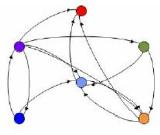
\includegraphics[scale = 0.4]{logoSoftVis.jpg}
        \end{wrapfigure}
O grupo tem como objetivo desenvolver metodologias , ferramentas e técnicas para visualização de software ( SoftVis ) e empiricamente caracterizar e avaliá-los. Tem o interesse especial no desenvolvimento de ambientes SoftVis que podem ser integrados para IDEs para reforçar atividades de compreensão de software e ajudar em tarefas de engenharia de software . Com esse objetivo , temos desenvolvido vários projetos.

\subsubsection{Sistemas de Tempo Real}
\begin{wrapfigure}{R}{0.3\textwidth}
            \centering
            
\includegraphics[scale = 0.4]{sterlogo.png}
        \end{wrapfigure}
Grupo de pesquisa focada no desenvolvimento de novas técnicas para a concepção, análise e implementação de sistemas de tempo real. O nosso grupo foi oficialmente certificada pela UFBA em maio de 2014. A nossa equipa tem vindo a investigar vários aspectos dos sistemas em tempo real , com especial ênfase no multiprocessador / multicore escalonamento de tempo real.

\subsubsection{ONDA DIGITAL - Grupo de Pesquisa e Extensão em Informática, Educação e Sociedade}
\begin{wrapfigure}{R}{0.3\textwidth}
            \centering
            
\includegraphics[scale = 0.2]{logoGPOndaDigital.png}
        \end{wrapfigure}
Grupo de Pesquisa e Extensão em Informática, Educação e Sociedade tem como eixo integrador as relações interdisciplinares entre Computação, Educação e Sociedade com especial interesse nas seguintes áreas: 
\begin{enumerate}
\item informática na educação; 
\item  interação humano-computador (teoria, desenvolvimento e avaliação de tecnologias interativas); 
\item educação em computação; 
\item informática, educação e sociedade.
\end{enumerate}

Desde 2004 o grupo tem estabelecido parcerias com a indústria de software, instituições educacionais e outros parceiros financiadores de projetos. Mais de 100 estudantes de graduação passaram pelo grupo ao longo dos últimos dez anos. Atualmente temos mais de 40 alunos, entre pesquisadores, estudantes de graduação, mestrado e doutorado.

\subsubsection{Computational Intelligence and Optimization Research Lab}
\begin{wrapfigure}{R}{0.3\textwidth}
            \centering
            
\includegraphics[scale = 0.2]{logos.png}
        \end{wrapfigure}
Inteligência Computacional é uma das áreas de Inteligência Artificial que lida com a aquisição de conhecimento automático. O nosso grupo está focado na teoria, aplicação e desenvolvimento de métodos de inteligência computacional .
	  
	  Optimização é uma das áreas de pesquisa operacional que lida com a encontrar as melhores soluções possíveis para os problemas . Nosso trabalho concentra-se na elaboração de teoria, modelos e algoritmos para problemas de optimização.